%=======================================================================
% Todos os códigos aqui são originais ou roubados de alguem!
% ------------------------------------------------------------------------
% ------------------------------------------------------------------------
% abnTeX2: Modelo de Trabalho Academico  em conformidade com 
% ABNT NBR 14724:2011: Informacao e documentacao - Trabalhos academicos
% ------------------------------------------------------------------------
%Customização para PPGDS - UNESC
% ------------------------------------------------------------------------
% Autor:  Fernando Alves Silveira
% Email: fernandoalvessilveira@gmail.com
% Versão: 20 de Julho 2020.
% Edição: TexStudio
% Codificação: UTF-8
% LaTeX:  abnTeX2
% 
%=======================================================================

\documentclass[
	% -- opções da classe memoir --
	12pt,				% tamanho da fonte	
	oneside,          % não imprimir em verso e anverso, oposto do twoside 
	a4paper,			% tamanho do papel. 
	% -- opções da classe abntex2 --
	chapter=TITLE,		% títulos de capítulos convertidos em letras maiúsculas
	section=TITLE,		% títulos de seções convertidos em letras maiúsculas
	subsection=TITLE,	% títulos de subseções convertidos em letras maiúsculas
	%subsubsection=TITLE,% títulos de subsubseções convertidos em letras maiúsculas
	% -- opções do pacote babel --
	english,			% idioma adicional para hifenização
	brazil			% o último idioma é o principal do documento
	,sumario=tradicional
	]{abntex2-unesc}


% ---
% Pacotes fundamentais 
% ---
\usepackage{cmap}				% Mapear caracteres especiais no PDF
\usepackage{times}			    % Usa a fonte Latin Modern			
\usepackage[T1]{fontenc}		% Selecao de codigos de fonte.
\usepackage[utf8]{inputenc}		% Codificacao do documento (conversão automática dos acentos)
\usepackage{lastpage}			% Usado pela Ficha catalográfica
\usepackage{indentfirst}		% Indenta o primeiro parágrafo de cada seção.
\usepackage{color}				% Controle das cores
\usepackage{graphicx}			% Inclusão de gráficos
\usepackage{amsfonts}			% Símbolos
%----Ajuste no alinhamento das listas
\usepackage{enumitem}
\setitemize[0]{itemindent=0.4cm,itemsep=0pt}
\setenumerate[0]{itemindent=0.5cm,itemsep=0pt}
%------
% ---
% Pacotes de citações
% ---
\usepackage[brazilian,hyperpageref]{backref}	 					  % Paginas com as citações na bibl

%Referência
\usepackage[alf, 	
			 		abnt-emphasize=bf,
				    abnt-url-package=none,
				    abnt-repeated-title-omit=yes,
				    abnt-full-initials=yes,                                        %yes nome por extenso, no apenas iniciais
					abnt-etal-list=3												%abreviar com mais de 3 autores
]{abntex2/abntex2cite}				 														    % Citações padrão ABNT
\usepackage{lipsum}							   								       % para geração de dummy text

%\captionsetup[table]{justification=raggedright}
% Configurações de aparência do PDF final
% alterando o aspecto da cor azul
\definecolor{blue}{RGB}{41,5,195}

% --- 
% Espaçamentos entre linhas e parágrafos 
% --- 
% O tamanho do parágrafo é dado por:
\setlength{\parindent}{2cm}
\linespread{1.5}

%Espaçamento depois dos títulos
\setlength{\afterchapskip}{\baselineskip}
% %\setlength{\afterchapskip}{\lineskip}

% Controle do espaçamento entre um parágrafo e outro:
\setlength{\parskip}{0cm}  % tente também \onelineskip

\hangcaption
\captionstyle[\raggedright]{}

%Estava mostrando nas referencias quais paginas estavam sendo referenciadas
\renewcommand{\backref}{}
\renewcommand*{\backrefalt}[4]{}

%Reduzir a fonte do caption
\captionnamefont{\ABNTEXfontereduzida}
\captiontitlefont{\ABNTEXfontereduzida}
%Ajuste nas listas de tabela, ilustrações e quadros
\setlength\cftbeforechapterskip{0pt}
% ---
% compila o indice
% ---
\makeindex
% ---

%----Include da capa é fora do documento 
% ---
% Informações de dados para CAPA e FOLHA DE ROSTO
% ---
\titulo{\textbf{TÍTULO: SUBTÍTULO SE HOUVER}}
\autor{\textbf{NOME DO ACADÊMICO}}
\local{\textbf{CRICIÚMA}}
\data{\textbf{2020}}
\orientador{Orientador 1 }
\coorientador{Coorientador 2 }
\banca{Membro da banca }
\instituicao{\textbf{UNIVERSIDADE DO EXTREMO SUL CATARINENSE - UNESC}}
\programa{\textbf{PROGRAMA DE PÓS-GRADUAÇÃO EM ......}}
\curso{\textbf{MESTRADO EM ......}}
\tipotrabalho{Tese ou dissertação)}
% O preambulo deve conter o tipo do trabalho, o objetivo, 
% o nome da instituição e a área de concentração 
\preambulo{Dissertação apresentada ao Programa de Pós-Graduação em ..... da Universidade do Extremo Sul Catarinense - UNESC, como requisito parcial para a obtenção do título de Mestre em .....}
\preambuloaprovacao{Esta dissertação foi julgada e aprovada para obtenção do Grau de Mestre em .... na área de ..... no Programa de Pós-Graduação em .... da Universidade do Extremo Sul Catarinense.}
% ---

%---

\begin{document}
% Retira espaço extra obsoleto entre as frases.
\frenchspacing 

% ----------------------------------------------------------
% ELEMENTOS PRÉ-TEXTUAIS
% ----------------------------------------------------------

%--- CAPA ----
\imprimircapa

% --- FOLHA DE ROSTO
\imprimirfolhaderosto
% \imprimirfolhaderosto* (o * indica que haverá a ficha bibliográfica)

% \imprime ficha catalográfica
\begin{fichacatalografica}
% Ficha catalografica de sugestão, vamos deixa para biblioteca da UNESC fazer alguma cosa.

    \vspace*{18cm}
    \fcolorbox{black}{white}{
    \begin{minipage}[c]{12.5cm}
    \vspace*{1cm} \\
    \centering
        A ficha catalográfica é confeccionada pela Biblioteca Central da UNESC. \\
        Tamanho: 7cm x 12cm \\
        Fonte: Times New Roman 10 \\
        Maiores informações em pelo e-mail biblioteca@unesc.net e \\             eliziane@unesc.net, ou pelo telefone 3431 4549. \\
    \vspace*{1cm}
    \end{minipage}
    }
    

    
\end{fichacatalografica}



% Inserir FOLHA DE APROVAÇÃO
\begin{folhadeaprovacao}

  \begin{center}
  \vspace*{-1.2cm}
    {\large\imprimirautor}

    \vspace*{\fill}
    {\large\imprimirtitulo}
    \vspace*{\fill}
    
    \hspace{.45\textwidth}
    \begin{minipage}{\textwidth}
    \vspace*{-7.cm}
        \imprimirpreambuloaprovacao
    \end{minipage}%
    \vspace*{\fill}
   \end{center}
    
  \begin{center}
  \vspace*{-5.cm}
  	 Criciúma, xx de ...... de 2020 (data da defesa)
  \end{center}
  \begin{center}
  \textbf{BANCA EXAMINADORA}
  \end{center}
  
  \begin{center}
  \vspace*{1.5cm}
   {\imprimirorientador     (Instituição) \\

    \vspace*{.5cm}
   \imprimircoorientador    (Instituição) \\

    \vspace*{.5cm}
   \imprimirbanca          (Instituição) \\


    }
    \end{center}
    
   \begin{center}
    \vspace*{3cm}
    {\large\imprimirautor}
    \par
    Mestrando
  \end{center}
  
\end{folhadeaprovacao}

% DEDICATÓRIA
\begin{dedicatoria}
 \vspace*{\fill}
 \noindent
  \raggedleft
 \begin{minipage}{.54\textwidth}
    Dedique este trabalho a quem você pensa ser merecedor.
   \end{minipage}
\end{dedicatoria}


% AGRADECIMENTO
\begin{agradecimentos}

\lipsum[1-1]


\end{agradecimentos}

%EPÍGRAFE
\begin{epigrafe}
    \vspace*{\fill}
	\begin{flushright}
		“Este espaço serve para você citar \\
		 um pensamento de algum autor que  \\
		 tenha relação com a temática do seu \\
		 trabalho. ”
		(Autor)
	\end{flushright}
\end{epigrafe}

% RESUMO
% resumo em português
\begin{resumo}
\noindent
Consiste na apresentação dos pontos relevantes de um texto. O resumo deve dar uma visão rápida e clara do trabalho; constitui-se em uma sequência de frases concisas e objetivas e não de uma simples enumeração de tópicos. Apresenta os objetivos do estudo, o problema, a metodologia, resultados alcançados e conclusão. Deve ser digitado em espaço simples e sem parágrafos, não ultrapassando a 500 palavras.
 %Aqui vai o resumo

 \vspace{0.2cm}

 
 \textbf{Palavras-chave:} Escrever de três a cinco palavras representativas do conteúdo do trabalho, separadas entre si por ponto e finalizadas também por ponto.
\end{resumo}

% resumo em inglês
\begin{resumo}[Abstract]	
 	\begin{otherlanguage*}{english}
 	\noindent 

	Resumo na língua inglesa. % Aqui vai o abstract

   \vspace{0.2cm}
 
   
    \textbf{Key-words:} Latex. Abntex. Text editoration.	
 	\end{otherlanguage*}
\end{resumo}

% lista de ilustrações
\pdfbookmark[0]{\listfigurename}{lof}
\listoffigures*
\cleardoublepage
% ---

% lista de quadros
% --- 
%PRECISO VER COMO FAZER O CONTROLE DE QUANDO TIVER MENOS Q 10 VAI PARA LISTA DE ILUSTRAÇÕES
\pdfbookmark[0]{\listofquadrosname}{loq}
\listofquadros*
\cleardoublepage
% ---

% LISTA DE TABELAS
\pdfbookmark[0]{\listtablename}{lot}
\listoftables*
\cleardoublepage  %-- força proxima pagina

% ---
% inserir lista de abreviaturas e siglas
% ---
\begin{siglas}
  \item[ABNT] Associação Brasileira de Normas Técnicas
  \item[PMC]  Prefeitura Municipal de Criciúma
\end{siglas}
% ---

% ---
% inserir lista de símbolos
% ---
\begin{simbolos}
  \item[$ \Gamma $] Letra grega Gama
  \item[$ \Lambda $] Lambda
\end{simbolos}
% ---

% SUMARIO
\pdfbookmark[0]{\contentsname}{toc}
\tableofcontents*
\cleardoublepage

% ------------------------------------------------------
% ELEMENTOS TEXTUAIS
% ------------------------------------------------------
\textual
% INTRODUÇÃO
% ----------------------------------------------------------
% Introdução
%Ex: \chapter{TÍTULO A SER IMPRESSO NO CORPO DO TEXTO}{Título no cabeçalho}{Título no Sumario}
% ----------------------------------------------------------
\chapter{INTRODUÇÃO} % se usar o \chapter* ele não vai colocar no sumario
%\addcontentsline{toc}{chapter}{Introdução} inclui manualmente no sumario sem numeração
Delimita o assunto, define brevemente os objetivos do trabalho e as razões de sua elaboração, bem como as relações existentes com outros trabalhos. Apresenta o problema e as questões norteadoras ou hipóteses. Não deve antecipar conclusões e recomendações.

\section{APRESENTAÇÃO}
Use este espaço para apresentar o tema e problema para seu leitor.

\section{DESCRIÇÃO DO PROBLEMA}
Descreva aqui seu problema de pesquisa.

\section{JUSTIFICATIVA}
Escreva aqui sua justificativa.

\section{OBJETIVOS}

\subsection{Objetivo geral}
Descreva aqui o objetivo geral a ser abordado pelo estudo apresentado.

\subsection{Objetivos específicos}
Desdobramento do objetivo geral. 
 \begin{itemize}
	\item Item 1
	\item Item 2
	\item Item 3
\end{itemize}

 \section{METODOLOGIA}
 
 Use este espaço para detalhar os procedimentos métodologico adotado.


%FUNDAMENTAÇÃO TEÓRICA
\chapter{FUNDAMENTAÇÃO TEÓRICA}

Apresentar estudos que contemple a temática abordada. Respeitar a autoria,
nas citações diretas e indiretas. Evitar parágrafos muito longos. Evitar seções e
subseções muito curtas.

\section{Exemplo de Seção}

Use este espaço para se apronfundar em sua fundamentação.

\subsection{Exemplo subseção}

Aproveita este outro espaço e se aprofunde ainda mais em sua teoria e bibliografia.

\subsubsection{Exemplo subsubseção}

Caso você ainda precise de mais profundidade, aproveite este espaço para detalhar pontos de seu interesse.


%DESENVOLVIMENTO
\chapter{DESENVOLVIMENTO}

Para \citeonline[p. 22]{minayo1994pesquisa}, “o conjunto de dados quantitativos e qualitativos não se opõem, ao contrário, se complementam.”Fica claro, então, que o objeto das Ciências Sociais é essencialmente qualitativo: a realidade social que “é o próprio dinamismo da vida individual e coletiva com toda a riqueza de significados dela transbordante.” \cite{minayo1994pesquisa}


\subsection{Tabela}

Tabelas podem ser criadas e inseridas facilmente com Latex. Elas podem ser personalidas. Colunas e linhas podem ser acrescentadas posteriormente. o Ajuste e flutuação pode ser indicado, entretant o Latex sempre procura a posição mais adequada.

\begin{table}[htb]
    \centering
    \caption{Pessoas residentes em domicílios particulares, por sexo e situação do domicílio – Brasil – 1980}
    \begin{tabular}{c c c c}
    \hline
        Situação do domicílio   & Total  &  Mulheres   &  Homens   \\
    \hline
        Total                   & 117.960.301 &  59.595.332 &  58.364.969 \\
        Urbana                  & 79.972.931  &  41.115.439 &  38.857.492 \\  
        Rural                   & 38.857.492  &  38.857.492 &  19.507.477 \\
    \hline
    \end{tabular}
    \fonte{Fundação Instituto Brasileiro de Geografia e Estatística - IBGE}
\end{table}


\subsection{Imagens}

A mesma flexibilidade aplicada para tabelas e gráficos pode ser empregada para introdução de imagens e figuras no texto. As boas práticas de uso do Latex indicam o uso de uma pasta determinada para guardar suas imagens e figuras.

\begin{fotografia}[htb]
 \IBGEtab{ %Comando nativo do pacote para geração dos labels das imagens e figuras
	\caption{Prática de Yoga na UNESC}
	\label{fot:grafico3}
 } {
  	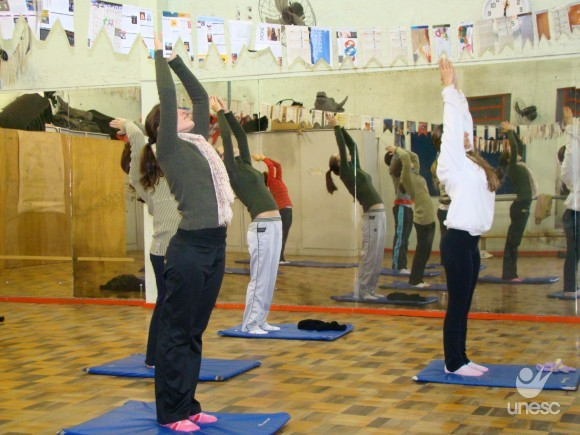
\includegraphics[scale=0.5]{figuras/yoga.png}
 } {
 	\fonte{Carrer (2004)}
 }
\end{fotografia}




%RESULTADOS
\chapter{RESULTADOS E DISCUSSÕES}

Aqui você apresenta os resultados obtidos e introduz ao leitor uma discussão sobre os resultados.



%CONCLUSÃO
\chapter{CONCLUSÃO}

Esta espaço é destinado para a apresentação de seus achados e contribuições acerca do tema.

% ----------------------------------------------------------
% ELEMENTOS PÓS-TEXTUAIS
% ----------------------------------------------------------
\postextual

% ----------------------------------------------------------
% Referências bibliográficas
% ----------------------------------------------------------

\bibliography{referencias}

%Apêndices
\begin{apendicesenv}

\chapter*{Título do Apêndice A}

Espaço destinado a apêndice e outros elementos pós textuais


\end{apendicesenv}

%Anexos
\begin{anexosenv}
\chapter*{Título do Anexo A}

Espaço destinado aos anexos e outros elementos pós textuais


\end{anexosenv}

\end{document}